\documentclass[a4paper]{article}
\usepackage[english]{babel}
\usepackage[utf8x]{inputenc}
\usepackage{float}
\usepackage{graphicx}
\usepackage{caption}
\usepackage{pmboxdraw}
\usepackage{color}
\usepackage{tocloft}
\usepackage[color]{vdmlisting}
\usepackage{longtable}
\usepackage[hidelinks]{hyperref} 
\usepackage{geometry}
\usepackage{amssymb}
\usepackage{array}
\usepackage{listings}
\geometry{a4paper, total={160mm,225mm}, left=25mm, top=35mm}

\definecolor{darkgray}{rgb}{0.41, 0.41, 0.41}
\definecolor{green}{rgb}{0.0, 0.5, 0.0}

\usepackage{listingsutf8}
\lstdefinestyle{JavaStyle}{
	language=Java, 	
	numbers=left,
	stepnumber=5,
	firstnumber=1,
	numberfirstline=true,
    basicstyle=\linespread{0.7}\ttfamily,
    keywordstyle=\color{blue}\ttfamily,
	showstringspaces=false,
    stringstyle=\color{red}\ttfamily,
    commentstyle=\color{green}\ttfamily,
	identifierstyle=\color{darkgray}\ttfamily,
	tabsize=4,
    breaklines=true,
    extendedchars=true,
	inputencoding=utf8x,
    escapeinside={\%*}{*)},
	frame=lines
}

\setlength{\tabcolsep}{6pt}
\setlength\cftaftertoctitleskip{20pt}
\begin{document}
%\setlength{\textwidth}{16cm}
%\setlength{\textheight}{22cm}


\title{
\includegraphics[scale=0.15]{feup_logo.png}
\linebreak\linebreak\linebreak\linebreak\linebreak
\Large\textbf{Research applied to the collection of waste in a city }\linebreak  {\large Final Report}
\linebreak\linebreak\linebreak\linebreak
\Large{Inteligência Artificial - 3\textsuperscript{rd} degree}
\linebreak
\Large{Mestrado Integrado em Engenharia Informática e Computação}\linebreak\linebreak\linebreak\linebreak
}
\author{\textbf{Turma 3 - Grupo A3\_2}\\
Artur Ferreira - ei12168 - ei12168@fe.up.pt\\
Nuno Valente - up200204376 - up200204376@fe.up.pt\\
\linebreak\linebreak \\
\linebreak\linebreak\linebreak
\linebreak\linebreak\vspace{1cm}}

\maketitle

\thispagestyle{empty}
\newpage
\tableofcontents 
\newpage

\section{Objective}
\label{objective}

This project aims to determine the best route to be performed by a collection of waste trucks in a city, and it has two main objectives: minimize the distance travelled on the route taken and maximize the load waste transported. The last objective relates to minimize the number of waste trucks that are involved.

\section{Description}
\label{description}

Waste collection is a daily task in a city that must be performed as efficiently as possible, either to keep the city clean or to minimize the associated costs. In order to transport waste to the treatment stations, the city services maintain a fleet of specialized lorries which carry out collection routes, that are defined previously and carried out systematically at a given frequency.

It is intended to perform such collection more intelligently. In fact, containers scattered in various parts of the city, where the residents deposit the garbage. These containers may not be full enough to justify emptying them by the collection truck, which would make some trips unnecessary. With the technology of sensor networks developing rapidly, more effective monitoring of the level of waste accumulation in each container is already possible.

We have considered the existence of 4 types of waste: paper, plastic, glass and ordinary trash. Each truck carries only one type of waste, because we must think in recycling.

In this work, we intend to develop an application that determines the collection routes to be made by trucks, considering only the containers with sufficient residue that justifies their collection. This application should be able to suggest the best route from the central, where the trucks are stationed, to the treatment stations, where all the collected waste is deposited.

As a first step, we have considered that the collection is carried out by a single truck of limited capacity. In a second phase, we'll consider several trucks with limited capacity and when trying to optimize the route, we want to use as few trucks as possible.

\section{Specification}
\subsection{Important concepts}

In this problem we need to consider a few concepts like truck, container, place of departure, the final place and the desired route. More properly:

\begin{itemize}
	\item The specialized truck has a limited capacity, a type of waste and a fuel diesel tank;
	\item The place of departure is the central where are the trucks to initialize their route;
	\item The final place is where, at the same time all the trucks have collected all the waste and leave their garbage in the treatment stations;
	\item One container is consider as a set of four individual type waste;
	\item The desired route is the itinerary that we're trying to determine considering the objective already mentioned. 
\end{itemize}

\subsection{Problem description}

In a summarized way, we need to determine the best itinerary that contemplates the already referred objectives in section \ref{objective}. The next subsections gather additional information necessary for the specification.

\subsection{Problem restrictions}

In order to make the problem more realistic, we had the intention in use real latitude and longitude coordinates of some streets of Porto where we put the containers, as we said we  would do in the previous report. But, to make the problem easier to debug we use fictitious distances stored in the nodes of the graph. 

Some restrictions were imposed in this problem:

\begin{itemize}
	\item We determine the cost associated to the utilization of each truck, taking only into account the diesel fuel spent on average by a normal lorry. 
	
	\item We assume a truck with infinity fuel but with a limited capacity with in their own container
	
	\item Doesn´t exist the agent truck driver, just only the truck
	
	\item Some limit values applied to some variables:
	\begin{description}
		\item Garbage container capacity(kg) $= 100$;
		\item Truck capacity(kg) $\in [0, 3000]$;
		\item Number of each type of truck $\in [1, 10]$;
		\item Minimum level of waste in a garbage container(kg) $\in [50, 100]$.
	\end{description}
		
\end{itemize}

\subsection{Problem representation}

To represent the map of this problem, we considered a undirected-weighted graph with a list of nodes. Each node has their adjacent edges and it is used to represent, in general, the garbage container map. More generally, a node represents a point of passage: a garbage container in some street, a treatment station, the central and a desactivated garbage container. 

Although it is possible to consult the entire project code in Annex \ref{source}, here we present the fields that appear in each of the structures necessary to represent the graph:

\iffalse 
In sense of mathematical settlement is represented by an unoriented graph G = (V, E), where V is
the set of vertices and E – a set of edges of the graph [1, 2]. The vertices of the graph correspond to
the selected crossroads. Most are crossroads of at least three streets, none of which is blind. The edges
of the graph correspond to the settlement streets that connect the vertices, and blind streets extending
from the streets. Such procedures are used to simplify the task. At Fig. 1 on the map of settlement
there were drawn vertices numbers (in circles) and edge numbers (in rectangles). Fig. 2 shows a graph
representing such model of the settlement.
The weights are assigned to the edge. They correspond to a total length of street, which is
represented by that edge. The length of each blind street is counted twice because the rubbish disposal
van has to pass it twice. The van have to pass once other streets, taking garbage, but it can pass them
any number of times passing to other streets. Such transfers have been called empty journeys. As
mentioned above, the optimal solution is one in which the sum made empty journeys and journeys to
landfill is minimal, because the length of the path travelled by the garbage truck affect on transport
costs and pollution of exhaust gases [11].



\fi

\begin{itemize}
\item Graph:
\lstinputlisting[firstline=9,lastline=15]{../../src/graph/Graph.java}
\item Node:
\lstinputlisting[firstline=11,lastline=18]{../../src/graph/Node.java}
\item Edge:
\lstinputlisting[firstline=4,lastline=7]{../../src/graph/Edge.java}
 
\end{itemize}


\subsection{List of requirements}\label{subsecsec:requirements}

In list of requirements above, in comparation with the same list in the previous report, we add a column with the field check to show what we had proposed to do when writing the previous report and what we actually did.
We can obvious observe that everythinh was implemented, the mandatory and the opcional tasks.

\begin{table}[H]
	\centering
	\label{tab:list-of-requirements}
	\begin{tabular}{ | m{2cm} | m{0.5cm} | m{2cm} | m{9cm} | }
		\hline
	\textbf{Check} &	\textbf{Id} & \textbf{Priority} & \textbf{Description} \\[2ex] \hline
		\centering \checkmark & R1 & Mandatory        & The user can chose the number of each type of truck available on the central \\ \hline
		\centering \checkmark & R2 & Mandatory         & The user can enter the truck capacity \\ \hline
		\centering \checkmark & R3 & Mandatory          & The user can select the number of stations to leave the garbage \\ \hline
		\centering \checkmark & R4 & Mandatory         & The user will see the result of the implemented search algorithm in console \\ \hline
		\centering \checkmark & R5 & Mandatory         & The application must provide the result with the data that the user chose to test \\ \hline
		\centering \checkmark & R6 & Opcional         & The user will see the result of the implemented search algorithm in a graphical friendly user interface. \\ \hline
		\centering \checkmark & R7 & Opcional         & Nodes and edges are loaded from a csv file to facilitate the edition of data \\ \hline
		\centering \checkmark & R8 & Opcional         & The user might chose other algorithms to find the best itinerary \\ \hline
	\end{tabular}
\end{table}

\subsection{Solution}\label{solution}

In order to finding the best solution to the problem, we have applied the algorithm $A^*$ to a object, namely AStarNode that represents some kind of photo, that is, the actual state on the seaarch algorithm. This algorithm figures the least cost path, starting their journey at the Truck Center - start state - and ending whenever all the trash is collected and deposited at a treatment station - the goal state. To chose the best AStarNode to $A^*$ algorithm uses a modified
evaluation function, the f function and a best-first search. The evaluation function f is an estimate of the value of a AStarNode x given by the following formula:


\begin{equation}\label{equation}
f(x) = g(x) + h(x)
\end{equation}

where $g(x)$ is the cost to get from the start state to state x and $h(x)$ is the estimated cost to get from state x to the goal state.

\subsubsection{The function $g(x)$}\label{cost_function}

In the equation refered in (\ref{equation}), the $g(x)$ represents the cost to reach the current position starting from the initial. 
To determine the cost we have calculate ... 

FINALIZAR

\subsubsection{The function $h(x)$}\label{heuristic_function}

In same way, the $h(x)$ is the heuristic function that is used to approximate distance from the current location to the goal state. This function is distinct because it is a mere estimation rather than an exact value. The more accurate the heuristic the better and faster the goal state is reach and with much more accuracy.
To determine the value of $h(x)$ where x is the actual state, we ...

To ensure the admissibility of the heuristic function $h(x)$, the distance
In a straight line between the geographic coordinates of the node in question
And the place of destination, only in the case where all places of interest
(POI) have already been visited. There are POIs with
Before it reaches the destination, the division into subproblems is used
With the allocation of POIs as intermediary places of destination, ensuring that The process described above is used. In advanced heuristics, online distance Between the geographical coordinates is multiplied by a factor (1.25),
Allowing in most cases, a lower generation of intermediate states,
Losing, however, the qualities of consistency and admissibility.
H1 (n) = (distanceT oGoal distanceRatio) +
(NeededLitersT oGoal priceRatio) (2)
H2 (n) = (1.25 distanceT oGoal distRatio) +
(NeededLitersT oGoal priceRatio) (3)
In the two heuristic functions, no estimates are made of expenditures
In hotels and tolls, as this is not possible.
Without significantly compromising the heuristic's admissibility.

FINALIZAR

\section{Development}

\subsection{Programming Languages, Tools, and APIs}

Both the algorithm and the graphical interface were programmed in Java with
support of the IntelliJ IDEA and Ecplise development environment programs. In the interface with the user we use Java Swing in the windows that allow the configuration of the application and to show some statistics. In map and solution view found, we embedded the dynamic modeling and analysis library of graphs GraphStream in Java Swing.

\subsection{Application structure}

The project is divided into four folders: diagrams(diagrams), source code (src), documents (doc) and resources (res). In order to organize the project source code, the files with the code sources are subdivided into six packets:

\begin{itemize}
\item Graph - representation of the problem map;
\item Gui - graphical interface that allows the simplified interaction of the program by the user.
\item Logic - problem solving logic search algorithms.
\item Tests - file that allows performing unit tests on important functions
from the program.

\end{itemize}

We provide some uml diagrams to better present some key packages in this project like logic\ref{lpdUML} and graph\ref{gpdUML}, and a module view of the project\ref{mvUML}, all in the \ref{annex}.

\subsection{Relevant details of implementation}

We were careful to choose the data structures that could be most effective in representing and manipulating data.


ACRESCENTAR


\section{Experiences}

In addition to the unit tests that test the important components of the program, experiments were also performed on the performance of the algorithm. We have used 3 graphs to test, with incremental number of nodes and edges, 3 heuristic functions, collectiong the following information, gathered in the table:

TABELA

\section{Conclusions} 

The application developed meets all the items of the list of requirements \ref{subsecsec:requirements}. 


We want to increment the number of nodes and edges, maybe try and test with other algorithm to compare the solutions. 


Cost minimization is important when planning routes serving the waste collection vehicles.
Influence on the amount of the costs of has among other length of the route. Garbage truck must pass
all the planned streets. Some of them must overcome a second time to get to the next street, now
without receiving waste.
This paper presents the method of determining the street, which must be passed more than one time
and the sum of their length is the smallest possible, which significantly reduces costs. The method
involves constructing a graph representing the streets of the settlement and extending it to the Euler's
graph in such a way that the sum of the length of the edges is minimal. Purpose is achieved by using
the theorem of Euler and clonal selection paradigm of artificial immune systems.
\section{Enhancements} 


It is suggested that in future works the way of generating / importing
Input data. Due to the difficult import of data with the format and
Details appropriate to the problem, it is advisable to make a
Of a large number of nodes and edges,
Size of the graph representing the map and consequently the complexity
Problems.

The next step in the planning garbage truck routes is an indication of the order of passing of
the streets. According to Euler theorem, such solutions exist. They can be obtained using for example
algorithms of Hierholzer or of Fleury or using the artificial immune systems. The presented algorithm
applies algorithm of Hierholzer.
Another issue is the division of the land in areas serviced by a fleet of vehicles, taking into account
their capacity and the amount of waste collected. This is a very important issue in connection to
the statutory changes relating to waste collection, which came into force this year in Poland. This issue
will be the target of further research of the author.

\newpage

\section{Resources}

\subsection{References}

\begin{enumerate}
	
	\item Slides from lectures classes
	\bibitem{lamport93}
	Stuart Russell, Peter Norvig
	\emph{Artifical Intelligence A Modern Approach},
	Pearson Education
	3rd edition,
	2010.
	\item \url{http://www.gpsvisualizer.com/tutorials/waypoints.html} 
	\item \url{http://junit.org/junit5/}
	

\end{enumerate}

\subsection{Used software} \label{openStreet}
\begin{enumerate}
	
\item \url{http://www.openstreetmap.org/}\label{itm:openStreet}
\item \url{http://jgrapht.org/}

\end{enumerate}

\subsection{Effective work of each group member}

Each element of the group, consisting of two students, initially worked on distinct parts of the project. As we were developing the project and advancing towards a final phase of it, we ended up working together because there was a fair division of the effort involved by each one. Thus, we agree on the following percentages:

\begin{itemize}
	
	\item Artur Sousa Ferreira - $50\%$
	\item Nuno Miguel Rainho Valente - $50\%$
	
\end{itemize}

\newpage
\appendix

\section{Annex}\label{annex}
\subsection{A Short User Manual}

\begin{center}
	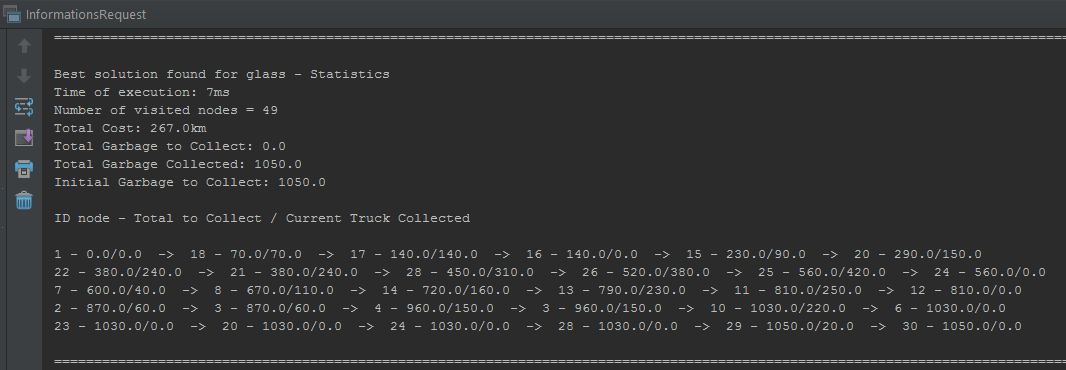
\includegraphics[scale=0.75]{console_statistics.png}
\end{center}
	
\subsection{Logic package diagram}\label{lpdUML}

\begin{center}
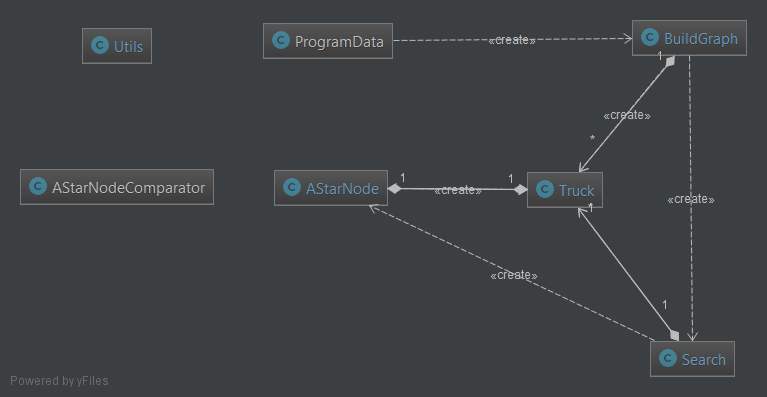
\includegraphics[scale=0.5]{../../diagrams/package_logic_diagram.png}
\end{center}

\subsection{Graph package diagram}\label{gpdUML}

\begin{center}
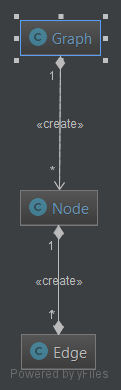
\includegraphics[scale=0.5]{../../diagrams/package_graph_diagram.png}
\end{center}

\subsection{Module View UML}\label{mvUML}

\begin{center}
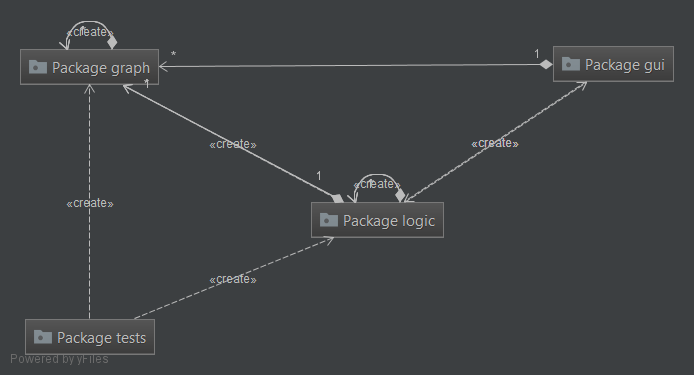
\includegraphics[scale=0.5]{../../diagrams/module_diagram.png}
\end{center}

\subsection{Graph examples used}\label{graphs}

\begin{center}\label{small_graph}
	\lstinputlisting{../../resources/graphs/small_graph.csv}
\end{center}

\begin{center}\label{medium_graph}
	\lstinputlisting{../../resources/graphs/medium_graph.csv}
\end{center}

\begin{center}\label{big_graph}
	\lstinputlisting{../../resources/graphs/big_graph.csv}
\end{center}


\subsection{Source Code}\label{source}
\subsubsection{Package graph}
\lstinputlisting[style=JavaStyle]{../../src/graph/Graph.java}
\lstinputlisting[style=JavaStyle]{../../src/graph/Node.java}
\lstinputlisting[style=JavaStyle]{../../src/graph/Edge.java}
\subsubsection{Package gui}
\lstinputlisting[style=JavaStyle]{../../src/gui/InformationsRequest.java}
\lstinputlisting[style=JavaStyle]{../../src/gui/Result.java}
\subsubsection{Package logic}
\lstinputlisting[style=JavaStyle]{../../src/logic/AStarNode.java}
\lstinputlisting[style=JavaStyle]{../../src/logic/AStarNodeComparator.java}
\lstinputlisting[style=JavaStyle]{../../src/logic/BuildGraph.java}
\lstinputlisting[style=JavaStyle]{../../src/logic/ProgramData.java}
\lstinputlisting[style=JavaStyle]{../../src/logic/Search.java}
\lstinputlisting[style=JavaStyle]{../../src/logic/Truck.java}
\lstinputlisting[style=JavaStyle]{../../src/logic/Utils.java}
\subsubsection{Package tests}
\lstinputlisting[style=JavaStyle]{../../src/tests/TestApp.java}
\end{document}